\FloatBarrier
\section{Results}
\label{sec:results}

The four predictions of Section~\ref{sec:cft:temporal} are now confronted with the simulations. All of them are measured on the ANNNI-type chain of Eq.~\eqref{eq:annni_H} at $\lambda=1$, quenched from $\ket{X+}^{\otimes N}$, with the frustration $p$ tuned from the integrable Ising point $p=0$ up to $p=0.5$. A window, in what follows, is the interval of evolution times over which a quantity can be fitted. It opens once $T$ is long enough for the conformal asymptotics to hold, and closes when the numerics stop resolving the object being fitted. The predictions split into two families, and this section follows that split. The entropy route goes through the eigenvectors: the generalized R\'enyi-2 entropy of Eq.~\eqref{eq:s2gen} is compared with the conformal profile of Eq.~\eqref{eq:cft:chord}. The spectral route goes through the eigenvalues alone. It carries three of the predictions: emergent dual unitarity, the central charge from the phase curvature of $\lambda_0$ (Eq.~\eqref{eq:cft:eq3}), and the boundary exponent from the first gap (Eq.~\eqref{eq:cft:eq4}). In each route the integrable point is measured first, where every prediction has an exact target~\cite{carignano_tagliacozzo2025}, and frustration is switched on afterwards.

Unless stated otherwise, all runs use the \textit{VD2} time-evolution MPO of Section~\ref{sec:mporep} with $\delta t=0.1$, the regulator $\beta_0=0.2$ ($N_\beta=4$, Section~\ref{sec:cft:boundary}), and the initial state $\ket{X+}$. The temporal states come from the block power method of Section~\ref{sec:numerics}, with $k=4$ at maximum bond dimension $\chi=64$ and larger blocks where the spectrum demands them---the deep spectra behind the boundary-tower measurements use $k=8$. Every eigenvalue-based measurement uses the measured sound velocity $v(p)$ of Appendix~\ref{app:velocity}.

\subsection{The entropy route}
\label{sec:results:validation}
\label{sec:results:wall}

At $p=0$ the generalized temporal entropy follows the conformal prediction over the full simulated window. Figure~\ref{fig:domes_p0} shows the R\'enyi-2 profiles: the real part collapses onto the chord curves of Eq.~\eqref{eq:cft:chord} with $c=\tfrac12$, and the imaginary part forms the predicted plateau. The plateau sits above $\pi c/16$ at every time we reach, and falls as $T$ grows, from $0.130$ at $T=4$ to $0.118$ at $T=15$. This is the finite-time correction that decays as $T^{-1/2}$~\cite{boucomas2026}. Fitting that form over $T=4$ to $15$ and extrapolating to infinite time gives $c=0.55$, an absolute estimate that needs no reference model.

\begin{figure}[htbp]
    \centering
    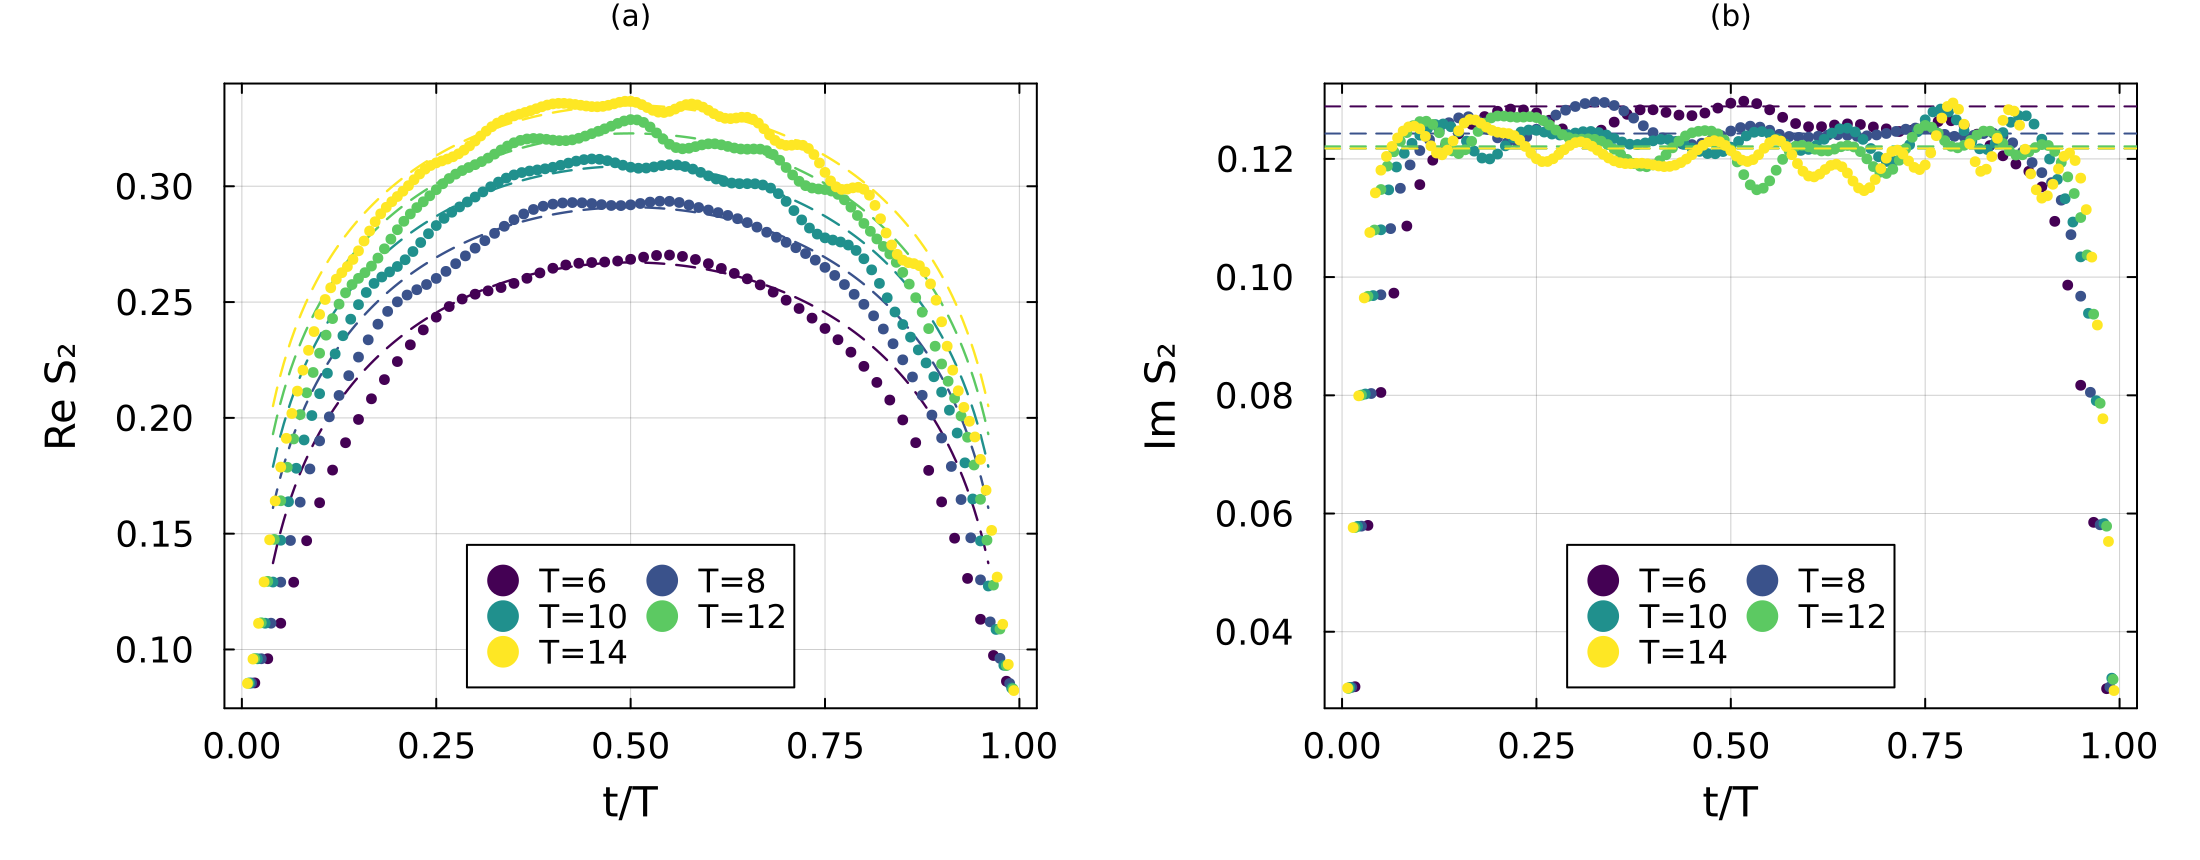
\includegraphics[width=\textwidth]{imgs/res_domes_p0.png}
    \caption{\textbf{The generalized temporal entropy at the integrable point.} One colour per evolution time. (a) Re $S_2$ against $t/T$. Each dashed curve is the prediction of Eq.~\eqref{eq:cft:chord} at $c=\tfrac12$ for that $T$, not a fit: its shape is fixed by the prediction, and only its height is matched to the data, since the additive constant $s_0$ is non-universal. What is being compared is therefore the shape. (b) Im $S_2$, flat across the interior of the strip as predicted. Each dashed line here is the measured plateau of its own $T$. The plateaus fall from $0.129$ at $T=6$ to $0.122$ at $T=14$, approaching the predicted $\pi c/16=0.098$ from above as the finite-time correction decays.}
    \label{fig:domes_p0}
\end{figure}

With frustration switched on, the entropy measurements are being regenerated on the corrected transfer-matrix column of Section~\ref{sec:mporep:exp}, and the frustrated windows and central charges of this route are \textit{[OPEN]}.

\subsection{The spectral route}
\label{sec:results:spectral}

The eigenvalue-only mode of Section~\ref{sec:blockpm} carries the spectral measurements to $T=20$ at $p=0$, the longest ladder we ran rather than a limit of the method. Figure~\ref{fig:spectral_p0}a traces $\lambda_0$ in the complex plane over that whole ladder: the modulus is constant at $1.487$ while the phase winds---the emergent dual unitarity of Section~\ref{sec:cft:temporal}. Figure~\ref{fig:spectral_p0}b shows the central charge from the same eigenvalue: the corrected fit of Eq.~\eqref{eq:cft:eq3} returns $c=0.48$. A longer window also improves the fit itself: with rungs out to $T=20$ the parameters of Eq.~\eqref{eq:cft:eq3} are individually resolved, and the constant term of Eq.~\eqref{eq:cft:eq3}, left free, converges to $B=-3.141$, matching the branch shift $-\pi$ expected from the definition $\lambda_0=\log(-\mu_0)$. The Casimir coefficient can also be checked against an independent calculation: for the critical Ising chain, where $c=\tfrac12$ and $v=2$ exactly, Eq.~\eqref{eq:cft:eq3} gives $|C|=\kappa/v=\pi c/(48)=\pi/96=0.0327$, the value obtained with a separate implementation of the method~\cite{boucomas2026}. We measure $|C|=0.0318$, within $3\%$.

\begin{figure}[htbp]
    \centering
    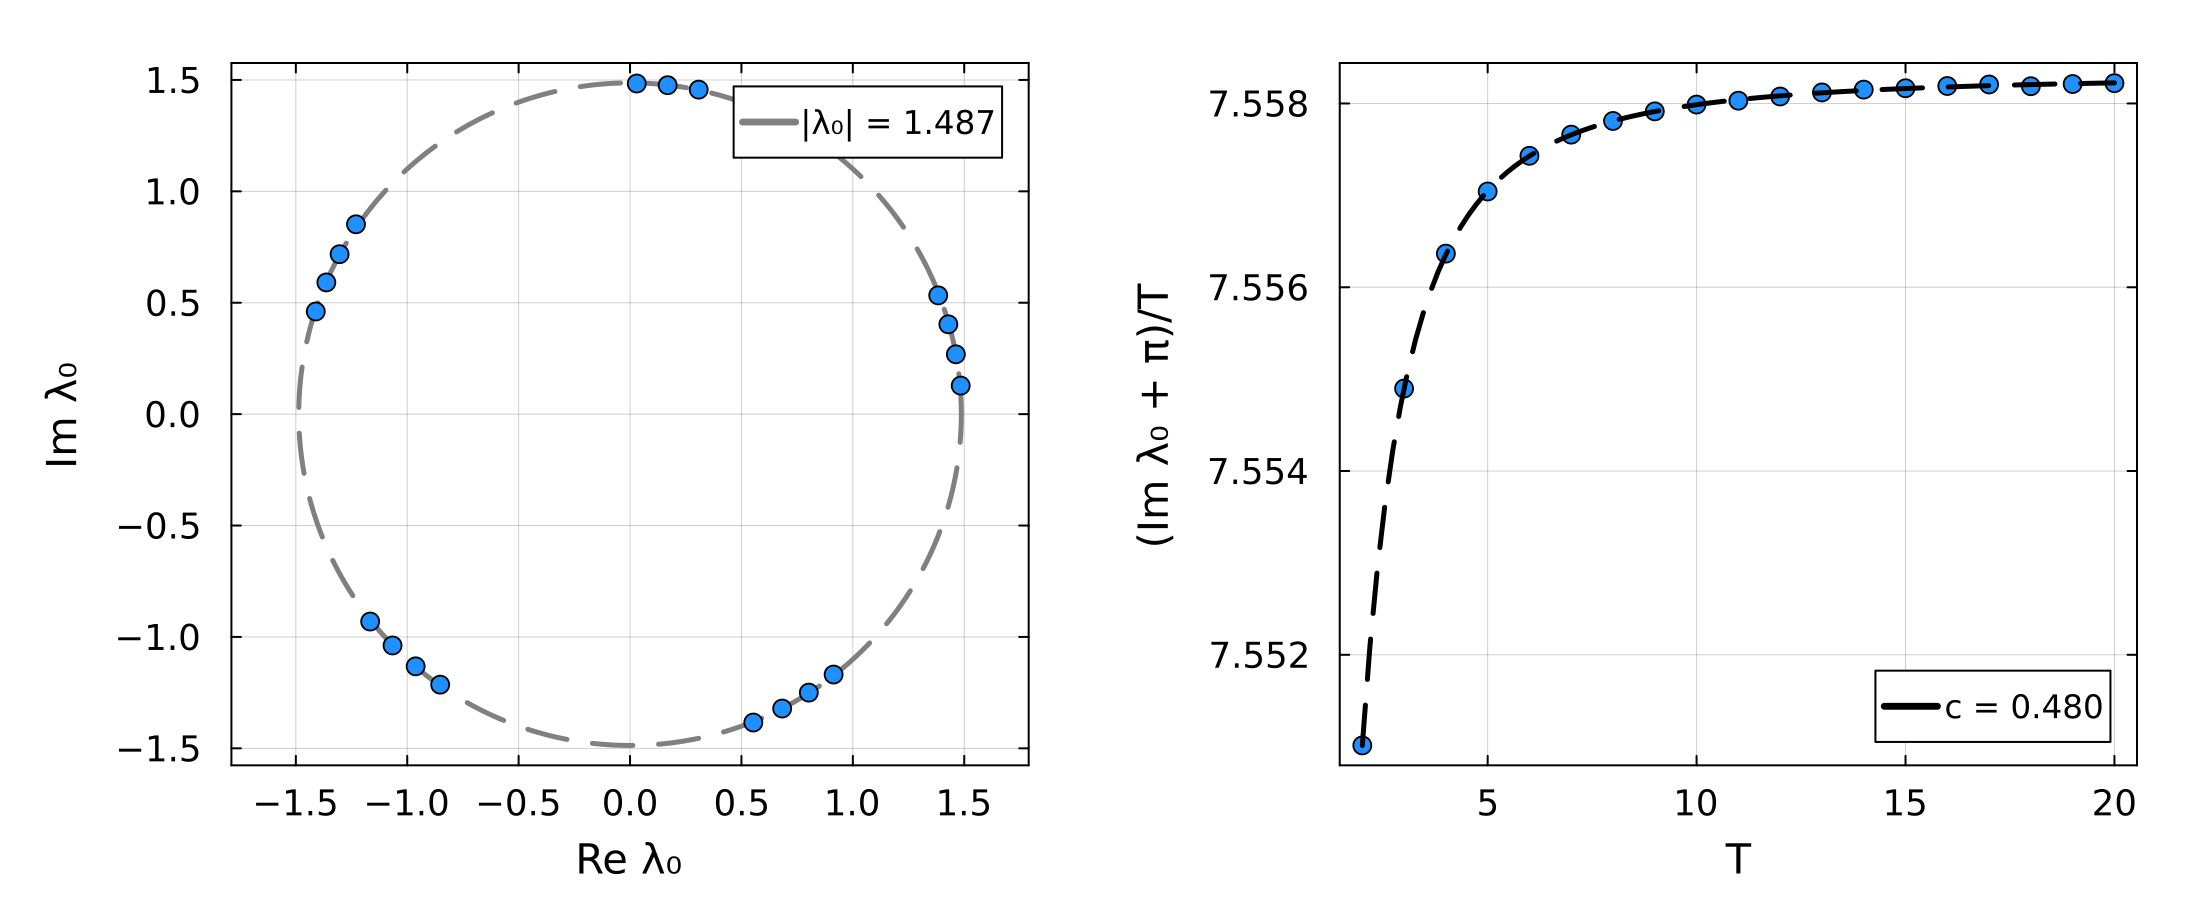
\includegraphics[width=\textwidth]{imgs/res_spectral_p0.png}
    \caption{\textbf{The spectral predictions at the integrable point, $T=2$--$20$.} (a) $\lambda_0$ in the complex plane: constant modulus, winding phase. (b) The fit of Eq.~\eqref{eq:cft:eq3} to $\mathrm{Im}\,\lambda_0$, plotted after subtracting the fitted extensive term $a_0T$ so that the small Casimir contribution is visible, giving $c=0.48$.}
    \label{fig:spectral_p0}
\end{figure}

The boundary exponent distinguishes the two boundary conditions of Section~\ref{sec:cft:temporal}. Fitting Eq.~\eqref{eq:cft:eq4} to the first spectral gap over $T=2$--$9$ gives $x_1=0.496$ for the free boundary ($\ket{X+}$) and $x_1=1.996$ for the fixed one ($\ket{Up}$), against the exact values $\tfrac12$ and $2$ (Figure~\ref{fig:x1_p0}).

\begin{figure}[htbp]
    \centering
    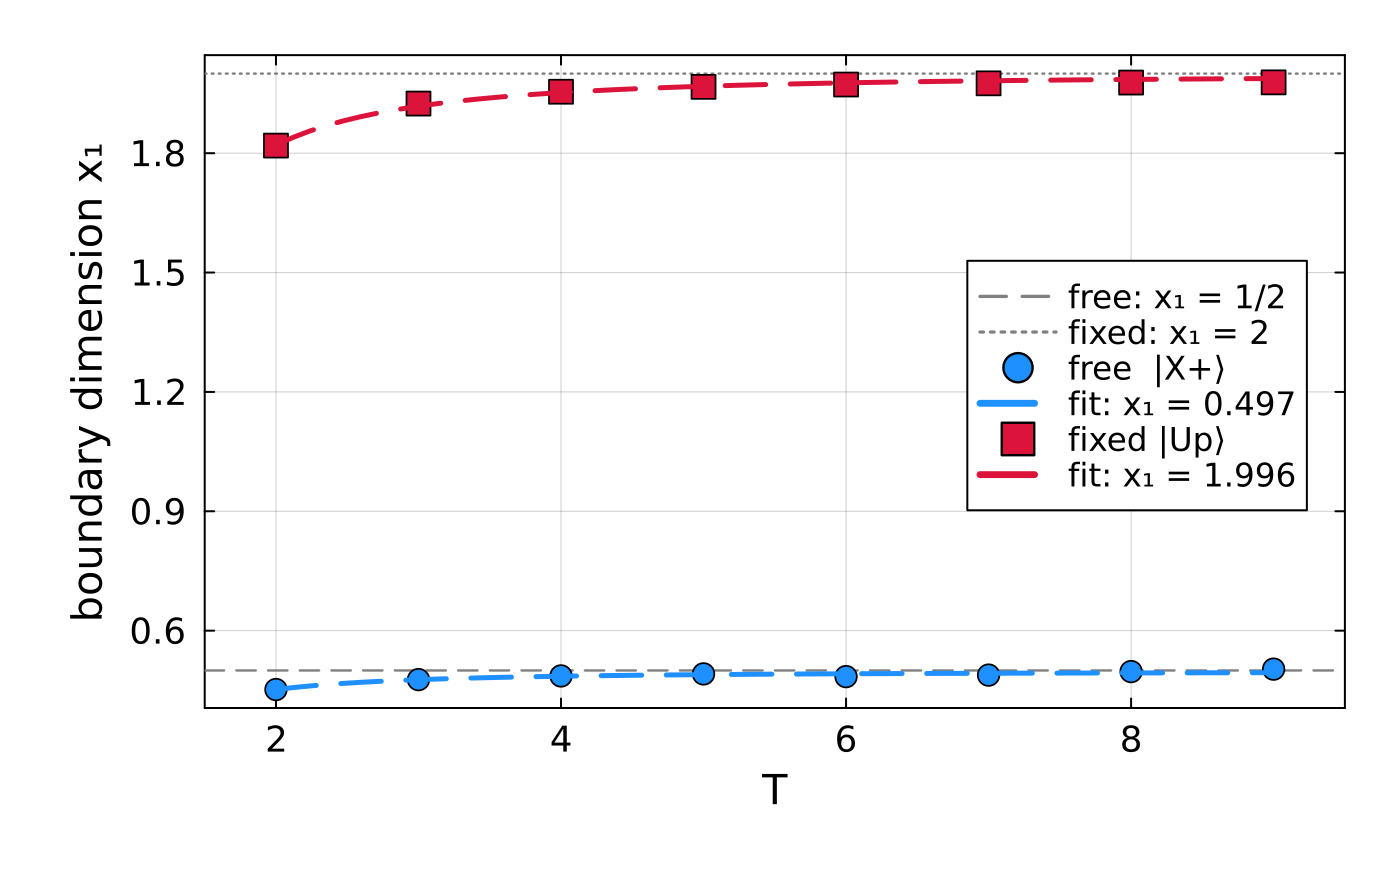
\includegraphics[width=0.65\textwidth]{imgs/res_x1_p0.png}
    \caption{\textbf{The boundary exponent at the integrable point.} The first spectral gap converted into a dimension, $x_1=v\,T\,\mathrm{Im}(\lambda_1-\lambda_0)/\pi$, against $T$ for the free and fixed boundary states. Grey lines mark the exact values $\tfrac12$ and $2$. Both approach their target from below as $T$ grows; the fits of Eq.~\eqref{eq:cft:eq4} over the whole window give $0.496$ and $1.996$.}
    \label{fig:x1_p0}
\end{figure}

At $p\neq0$ the spectral ladders are being regenerated on the corrected column, and the central charges and boundary exponents at the frustrated couplings are \textit{[OPEN]}. The resolution they demand is fixed in advance by Eq.~\eqref{eq:cft:eq4}: every boundary dimension is read from a phase gap of order $\pi x/(v\,T)$, so raising $p$ from $0$ to $1.5$ raises the velocity from $2.00$ to $10.80$ and compresses the same operator content into a phase window five times narrower. Table~\ref{tab:cp} collects the universal data measured so far.

\begin{table}[!htbp]
    \centering
    \begin{tabular}{lccc}
    \hline
    $p$ & R\'enyi-2 slope $c$ & eigenvalue-route $c$ & boundary exponent $x_1$ \\
    \hline
    $0$   & $\tfrac12$ (calibration) & $0.485$ & $0.496$ \\
    $0.1$ & \textit{[OPEN]} & \textit{[OPEN]} & \textit{[OPEN]} \\
    $0.3$ & \textit{[OPEN]} & \textit{[OPEN]} & \textit{[OPEN]} \\
    $0.5$ & \textit{[OPEN]} & \textit{[OPEN]} & \textit{[OPEN]} \\
    $1.0$ & \textit{[OPEN]} & \textit{[OPEN]} & \textit{[OPEN]} \\
    $1.5$ & \textit{[OPEN]} & \textit{[OPEN]} & \textit{[OPEN]} \\
    \hline
    \end{tabular}
    \caption{\textbf{Universal data versus frustration.} The integrable point is measured on ladders reaching $T=20$ and agrees with the exact Ising values. The frustrated rows are being regenerated on the corrected transfer-matrix column and remain open.}
    \label{tab:cp}
\end{table}
